\documentclass[12pt,twoside]{report}
\usepackage[a4paper,width=150mm,headheight=110pt,top=25mm,bottom=25mm]{geometry}
\usepackage[utf8]{inputenc}
\usepackage{listings}
\usepackage{graphicx}
\usepackage{mathdots}
\usepackage{tikz}
\usepackage{pgffor} 
\usepackage{float}
\usepackage{graphics} 
\usepackage{fancyhdr}
\usepackage[round, numbers,authoryear]{natbib}
\usepackage{color}
\usepackage{indentfirst}
\usepackage{epigraph}
\usepackage{ragged2e}
\usepackage{blindtext}
\usepackage{amsmath,amsthm,amssymb}
\usepackage{tabto}
\usepackage{pgfplots}
\usetikzlibrary{arrows.meta}

\graphicspath{{images/}}

\definecolor{mycolor}{RGB}{30,75,180}
\definecolor{mycolor2}{RGB}{40,75,90}
\definecolor{red}{RGB}{200,0,0}
\usepackage[colorlinks = true,
            linkcolor = mycolor,
            urlcolor  = mycolor,
            citecolor = mycolor,
            anchorcolor = mycolor]{hyperref}

\usepackage[hypcap=true,font={small,it}]{caption}
\usetikzlibrary{calc}

\captionsetup{belowskip=2pt,aboveskip=2pt}
\bibliographystyle{abbrvnat}

\renewcommand{\chaptername}{}

\renewcommand{\figureautorefname}{figure} % lower case default ref
\renewcommand{\tableautorefname}{table} % lower case default ref
\newcommand{\latex}{\LaTeX\xspace}
\newcommand{\mcite}[1]{\textcolor{mycolor}{\citeauthor{#1} (\citeyear{#1})}}
\newcommand{\hcite}[1]{(\textcolor{mycolor}{\citeauthor{#1}, \citeyear{#1}})}
\newcommand{\defi}[1]{\textbf{#1}}
\newcommand{\naming}[1]{\textbf{#1}}
\newcommand{\todo}[1]{\textbf{\color{red} TODO: #1}}
\newcommand{\gam}[2]{\mbox{$\{#1\:|\:#2\}$}}
\newcommand{\Gm}[1]{\mbox{$G#1$}}
\newcommand{\Hm}{\mbox{$H$}}
%----------------------------------------------------------------------------------------------------%

%--------------------------------------------- DOCUMENT ---------------------------------------------%
\begin{document}
%\fancyhead[RO,LE]{}
% Title page
    \begin{titlepage}
\vspace*{-2.5cm}
\begin{figure}[H]
    \hspace*{-1.0cm}
    \vspace*{-0.5cm}
    
\includegraphics[scale=0.4]{images/logo_ime.png}\\
\end{figure}

\noindent Universidade de São Paulo - Instituto de Matemática e Estatística\\
Bachelor's Programme in Computer Science
    \begin{center}
        \vspace*{1cm}
        
        {\LARGE \textbf{HOT GAMES}}
        
        \vspace{0.5cm}
        Temperature, advantage and numbers
        
        \vspace{1.5cm}
        by \\
        \vspace{1.5cm}
       Matheus Tararam de Laurentys
                
        \vspace{1.0cm}
    \end{center}

\noindent{
\textcolor{red}{{\bf Abstract} (The Abstract is a short summary of what your thesis is about. It accurately reflects the content of the thesis providing information about the research problem, research aims, methods and procedures, results and implications. It is a short section. Abstracts give readers the opportunity to quickly see the main contents of the paper and enable them to decide whether the paper is of particular interest to their needs. This section will be one of the last sections that you write. No subheadings are used in an abstract.)
}
}
\vfill
\textcolor[rgb]{0.5,0.5,0.5}{
    \begin{flushleft}
    { \small
    MAC0499 \\
    Undergraduate Thesis \\
    (Month) (Year) \\
    Supervisor: José Coelho Pina \\
    }
    \end{flushleft}
}
      
\end{titlepage}

% Optional Chapters

    %\chapter*{Dedication}
    %\chapter*{Declaration}
    \chapter*{Acknowledgements}
    \textcolor{red}{It is usual, but not compulsory, to thank those who have been of particular help to you in completing the thesis.}

% Table of contents, list of figures, and list of tables
    {\hypersetup{linkcolor=black}
        \tableofcontents
        \listoffigures
        \listoftables
    }
        {\hypersetup{linkcolor=mycolor}}
    
% Introduction
    \chapter{Introduction} 
    \renewcommand{\textflush}{flushepinormal}
\setlength\epigraphwidth{.8\textwidth}
\epigraph{``I learned very quickly that playing games and working on mathematics were closely intertwined activities for him, if not actually the same activity. His attitude resonated with and affirmed my own thoughts about math as play, though he took this attitude far beyond what I ever expected from a Princeton math professor, and I loved it."}{Manjul Bhargava \footnotemark}

\footnotetext{Fields medalist commenting on John Horton Conway's passing}



It is no surprise that avid players of games that resemble logical or
mathematical puzzles, like checkers, develop an intuition that allows
them to calculate faster. This intuition comes in many forms like
asserting bad moves fast and recognizing losing, drawing and winning
patterns. A most essential, and sometime very hard, component of
playing well any of these mathematical games is being able to know if
you are ahead or behind in a given position.

%%%%%%%%%%%%%%%%%%%%%%%%%%%%%%%%%%%%%%%%%%%%%%%%%%%%%%%%%%%%%%%%%%%
% mensagem caso 1 jogo não é suficiente para caso n jogos
%%%%%%%%%%%%%%%%%%%%%%%%%%%%%%%%%%%%%%%%%%%%%%%%%%%%%%%%%%%%%%%%%%%
While asserting which player a position favors is already a hard task,
this ability is not enough to play well in the games this text
showcases. Consider the following variant of the game of chess: each
player is given a set of board positions, and each should choose one
board to play as white. During this game, play will take place in each
board in parallel, and, whoever checkmates the opponent faster, wins
the game. If one wants to be a great player of this variant, asserting
if a position is winning or loosing in a regular chess game is not
enough, nor is the ability to play regular chess perfectly.

The most important ability for this ``parallel'' variant, 
and for the games that this text focus on, is
to score each position.
%%%%%%%%%%%%%%%%%%%%%%%%%%%%%%%%%%%%%%%%%%%%%%%%%%%%
Scoring a position is different from spotting which one
is better from a range of options.
%%%%%%%%%%%%%%%%%%%%%%%%%%%%%%%%%%%%%%%%%%%%%%%%%%%
To simplify, for these first few pages, the reader can
regard scoring as labeling a position with a real number.
%%%%%%%%%%%%%%%%%%%%%%%%%%%%%%%%%%%%%%%%%%%%%%%%%%%%%%%
If one can label different position in chess, and
these labels reflect advantage, 
then playing the proposed variation becomes easy.
%%%%%%%%%%%%%%%%%%%%%%%%%%%%%%%%%%%%%%%%%%%%%%%%%%%%%
In this day and age, making a 
classifier that performs well is chess,
or the proposed variant, and
many other games of this sort is a reality.
%%%%%%%%%%%%%%%%%%%%%%%%%%%%%%%%%%%%%%%%%%%%%%%%%%%%%%%%%%%%
However, a method to perfectly classify, or at least proving
a position is better than another, is not widespread.
 
The ability to precisely calculate the advantage a player has in a
position is the object of interest of Combinatorial Game Theory.
%%%%%%%%%%%%%%%%%%%%%%%%%%%%%%%%%%%%%%%%%%%%%%%%%%%%%%%%%%%%%%%%
This theory provides means of labeling all positions in games, not
just in chess, but in all combinatorial games.
%%%%%%%%%%%%%%%%%%%%%%%%%%%%%%%%%%%%%%%%%%%%%%%%%%%%%%%%%%%%
A position in Go and a position Checkers, two different games,
might have the same label and that means they are both equally
good or bad. The modern approach to combinatorial games
was inaugurated in~1976 in the book
\textit{On Numbers And Games}\cite{ONAG1}, but there are studies that date
back from the 1930s~\cite{CGT}.
%%%%%%%%%%%%%%%%%%%%%%%%%%%%%%%%%%%%%%%%%%%%%%%%%%%%%%%%%%%%
The author of that book, Jonh Horton Conway, as
found in the epigraph that starts this text, was, as many, an avid
player of such games.
%%%%%%%%%%%%%%%%%%%%%%%%%%%%%%%%%%%%%%%%%%%%%%%%%%%%%%%%%
In fact, Conway tells that the event that led to
him invent, or discover, this theory was watching two Go players
playing an endgame.

Conway realized that some positions
behaved like numbers, in every aspect.
%%%%%%%%%%%%%%%%%%%%%%%%%%%%%%%%%%%%%%%%%%%%%%%%%%%%%%%%%%
While, initially, that seems very useful to evaluate games,
Conway went ahead and proposed that some positions \textbf{are}
numbers.
%%%%%%%%%%%%%%%%%%%%%%%%%%%%%%%%%%%%%%%%%%%%%%%%%%%%%%%%%%
There is a  difference between label an object
as a number and an the object \textit{being} that number.
%%%%%%%%%%%%%%%%%%%%%%%%%%%%%%%
The key point in Conway's ideia is
that one can define operations as addition
such that the sum of two games
\textit{is} the sum of the numbers they are equal to.
%%%%%%%%%%%%%%%%%%%%%%%%%%%%%%%
The beautiful thing about games is that the sum is defined
in the most natural way.
%%%%%%%%%%%%%%%%%%%%%%%%%%%%%%%%%%%%%%%%%%%%%%%%%%%%%%%%%%%%
PARAMOS AQUI
%%%%%%%%%%%%%%%%%%%%%%%%%%%%%%%%%%%%%%%%%%%%%%%%%

%%%%%%%%%%%%%%%%%%%%%%%%%%%%%%%%%%%%%%%%%%%%%%%%%%%%%%%%%%
Later the reader will be presented to the  idea that
integer numbers are games, fractions are games, reals are games,
and many more numbers are also games.
%%%%%%%%%%%%%%%%%%%%%%%%%%%%%%%%%%%%%%%%%%%%%%%%%%%%%%%%%
This match is further explained in the
following chapters and is the main topic in this
field of study.

As stated before, there are games that are numbers, but not real. In fact the games that are numbers formed a new set, to be analyzed in the next sections. These numbers will not look like numbers at first. However, after visiting how they add up together in the most natural way, how they form an enormous set from extremely simple rules and other great characteristics, like being a completely ordered set, the reader might start appreciating them. The Surreal Numbers\footnote{Originally Conway only called them numbers, but greatly appreciated the name given by Knuth}, name given by Donald Knuth in \textit{Surreal Numbers: How Two Ex-Students Turned on to Pure Mathematics and Found Total Happiness}\cite{SN}.

As some might understand from the title alone, however, the focus of this text are in the non-numbers. It is possible for games to not behave like any of the surreal numbers, although every surreal number has correspondent\footnote{There are infinite games that are equal to any Surreal Number} games. The concept of temperature, and by consequence all the simpler concepts like hotness and coolness, however, does not forego the understanding of numbers. The reader will find that all games become numbers after some moves, so understanding them is paramount.

After a vista on both numbers and non-numbers, this text has two chapters targeted on exercising the concepts learned, visiting fun games to play and proofs on classes of games, including a new result from 2019 which is the first of its kind. The text as a whole will make the case that Combinatorial Game Theory is built upon extremely simple but powerful concepts. The few concepts are considered powerful because they not only provide a vast field of problems but allow simple proofs for them as well.

The next three sections will present the basics of Combinatorial Game Theory, describing numbers and non-numbers. The style of these sections will be similar to that of the book \textit{Winning Ways for your Mathematical Plays}\cite{WW}. It means that concepts, notation and theorems are not highlighted or enumerated and, instead, their meaning are presented in the regular paragraphs. This style fits well a text in Combinatorial Game Theory because most most of them are extremely simple and only a few of them are abstract. In this field, it is easy to write examples of the concepts so there is no necessity of abstracting as much as other areas of algebra or combinatorics.

The style of the book is also widely known for being non-rigorous where it does not have to be. The book will commonly use images of games that satisfy assertion and provide, or not, a logic why other games also satisfy that, without a rigorous proof. This is not followed as much in this text, justifications may be provided where not required. 

On the other side of the spectrum there is \textit{Combinatorial Game Theory}\cite{CGT}. Siegel is likely the most active researcher of the field nowadays and created the most developed tool used to analyze them, CGSuite. CGSuite is an very useful tool and more about it may be found in appendix A. Unlike the authors of \textit{Winning Ways for your Mathematical Plays}, he gave a great deal of form to this field. The book contains hundreds of definitions, notations, theorems and lemmas which are all enumerated and highlighted. One of the results is that his standards became widely used and that helps reading current papers. In general the book is more advanced and is the primary reference for chapters 5 and 6.

Between the two there is the book \textit{On Numbers and Games}\cite{ONAG1}\cite{ONAG2}, and possibly all others. The first edition of the book, as stated before, gave birth to the modern approach of Combinatorial Game Theory. The book is much more theoretic and focused on pure mathematics, containing much more algebra and number theory, than the successors, but is also extremely descriptive. There are other great books, but almost all the content of this text references only these three books.

Lastly, it may be worth observing that the text does not, nor does it intend to, contain everything there is in the field. In fact, it does not even shows everything there is about hot games. It may, however, serve as reference to short partisan games and will bring all the fundamental concepts of this class of games. There is a list of content that was omitted and approaches that were not discussed in the final chapter. Notice, however, that short games form a massive class of games and many of the fun games are short, so studying them first is typical, and hopefully it sparks interest in the remaining areas of the field.














    
% Definitions
    \chapter{What to do with pen, paper and a friend}
    %\chapter{Pen, Paper, a Friend and the Rules}
    
In order to study mathematical plays and answer the many questions they raise a new mathematical field of study was developed and many new terms were created. The phrase "mathematical play" is in itself a new term, for instance. While the most common term is "Combinatorial Games", the canonical reference for this field \textit{Winning Ways for Your Mathematical Plays} 1981, uses the former, not the latter. As more is said about the topic, more meaning the term "mathematical play" is going to acquire.

The name ``Combinatorial Game" might bring to light some information. It, at least, means that this field will deal with games, as in, an instance of a Game Theory problem, and, more specifically, a subset of those games. It also brings to light that the use of counting, finite structures and, most likely, graph representations will be heavily used (combinatorics). However, a definition of the object of interest becomes possible with the name mathematical play.

To play something mathematical could be understood as to engage in an activity in which the better use of mathematical ability, such as counting and logic, would result in advantage over its poor use. However it could be detailed further to an activity in which mathematical ability is the single defining factor. The later might make more sense because there are games, like poker, that do require some counting ability; however, luck and reading behavior skill are much more valuable to a successful game and this is something the definition would be better off forbidding.

\defi{Chance moves}, like throwing a dice or flipping a card, are not fit for mathematical plays. Even with their removal, however, there are possibilities that would not me comfortably called mathematical plays. The nature of a mathematical plays is that both players can engage the same activity and generate advantages out of "good play". For instance, it would be hard to agree that two people play rock-paper-scissors are battling a mathematical fight (even though there are no chance moves).

It is very important that all players have \defi{complete information} of the position. Games like rock-paper-scissors, in which players take action simultaneously, block complete information. Therefore, players must \textbf{move alternately}. The last concerning factor in discerning mathematical from non-mathematical plays during this analysis is the number of players.

When each player has more than one opponent a greater goal (than gaining advantage) arises. When playing with over two people it is frequent that the best move is not the one that brings  a better position but one that prevents any of the opponents from gaining an winning advantage. While that can be very mathematical, there is a clear distinction between sticking to two player games and allowing any number of players (notice that one can consider soccer as a two player game - even though there are multiple agents in a team). In order to focus on the mathematical ability to make the best move, the option to allow only \textbf{two players} is the most interesting.

The only remaining criteria of this definition (as established in [\todo{WW}]), that is related to the term play, and not the term mathematical, is preventing an infinite game. The rules of the game must guarantee that from any starting position, \defi{\todo{play should always} end because a player will not have moves available}. If following "\defi{normal play}" convention, a player that cannot move is lost. It is  correct to assume normal play, unless specified otherwise, in this field of study.

The foundations of mathematical plays, highlighted, give light to a complex and rich set of problems. At the same time, some other complex and rich problems are left behind. The game of chess, for example, does not meet the ending condition and, therefore, is left out. Fortunately, games like chess might benefit from these studies to adaptations or additional rules (although they do not consist of good examples of combinatorial games). Take the following example:\\

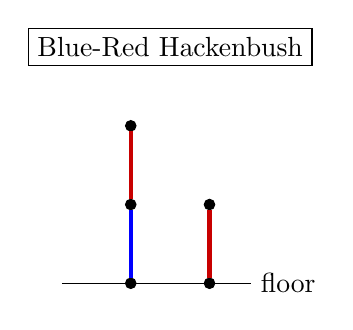
\begin{tikzpicture}
	\node[draw] (title) at (1.5, 3) {Blue-Red Hackenbush};
	\node (p1) at (0,0) {};
	\node (p2) at (3,0) {floor};
	\begin{scope} [every node/.style={scale=0.4, circle, draw, fill=black}]
		\node (p3) at (1,0) {};
		\node (p4) at (1,1) {};
		\node (p5) at (1,2) {};
		\node (p6) at (2,0) {};
		\node (p7) at (2,1) {};
		\draw (p1) -- (p2);
		\begin{scope} [ultra thick]
			\draw[blue] (p3) -- (p4);
			\draw[red] (p4) -- (p5);
			\draw[red] (p6) -- (p7);
		\end{scope}
	\end{scope}
\end{tikzpicture}


In this game, a move is made by taking a single colored edge of the image and removing any edges that become disconnected from the floor. One player can only remove blue edges, and the other, red edges.

It is a common practice to assume that, unless specified otherwise, games will be played between the players \naming{Left (bLue)} and \naming{Right (Red)}.




% Theory
    \chapter{Numbers are games. The reals, the cardinals and many others.}
    \epigraph{``And behold! When the numbers had been created for infinitely many days, the universe itself appeared. And the evening and the morning were the $\aleph^[\footnotemark^]$ day. And Conway looked over the rules he had made for numbers, and saw that they were very, very good. And he commanded them to be for signs, and series, and quotients, and root. Then there sprang up an infinite number less than infinity. And infinities of days brought forth multiple orders of infinities"}{Donald Ervin Knuth, Surreal Numbers \footnotemark}

\footnotetext[1]{In order to match the the cardinal number notation, it would be more precise to write $\aleph_0$. The text will use the book notation $\aleph$.}

\footnotetext{Excerpt of the book \textit{Surreal Numbers: how two ex-students turned on to pure mathematics and found total happiness} that precedes the moment the couple define a rule for addition of numbers.}


Conway, by counting the number of spare moves a player has in combinatorial games, unveiled a new way to discover numbers. It is clear at this point that although numbers are not enough to represent games, they are the building blocks of all games, including the non-numbers. Until this point, the text showed some instances of the zero and hinted at $1$ and $-1$, and the reader may also guess on how to build any integer in RB-Hackenbush and Domineering. This chapter shows that knowing that is no more than scratching the surface of surreal numbers.

For the first parts of this section a number \gam{x_1, x_2,\, $\ldots$}{y_1, y_2,\,$\ldots$} might be called like a real number: $2, 5, 100000, \frac{1}{3}, \sqrt{10}, \pi$, but there is no reason believe this equality yet. There is also no reason to believe that $1 < 3$ or that $1 + 1 = 2$ yet. Up until this point, numbers are labels to games that trivially translated the number of spare moves a player has. However, first a few more numbers will be labeled and only then the operations and comparisons are defined.


\subsection*{Numbers Generated in Finite Steps}

It is known that \Gm{} =
\begin{tikzpicture}
	\draw[] (0.3,-0.3) rectangle ++(0.3,0.3);
	\draw[] (0,-0.3) rectangle ++(0.3,0.3);
\end{tikzpicture} = \gam{}{\gam{}{}} = \gam{}{0} and \Gm{} was labeled $-1$.
What would be a good label for \Hm = 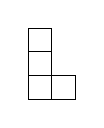
\begin{tikzpicture}
\draw[] (0.3,-0.3) rectangle ++(0.3,0.3);
\draw[] (0,-0.3) rectangle ++(0.3,0.3);
\draw[] (0,0) rectangle ++(0.3,0.3);
\draw[] (0,0.3) rectangle ++(0.3,0.3);
\end{tikzpicture}, given that it must be meaningful like described previously?\\ If it were to be labeled by a real number, which one should it be?

It is possible to find out a candidate by calculating \Gm{ + \Hm + \Hm}. To do that, one would usually find the game tree of 
\Gm{ + \Hm + \Hm} = 
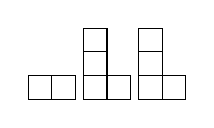
\begin{tikzpicture}
	\draw[] (-0.4,-0.3) rectangle ++(0.3,0.3);
	\draw[] (-0.7,-0.3) rectangle ++(0.3,0.3);
	\draw[] (0.3,-0.3) rectangle ++(0.3,0.3);
	\draw[] (0,-0.3) rectangle ++(0.3,0.3);
	\draw[] (0,0) rectangle ++(0.3,0.3);
	\draw[] (0,0.3) rectangle ++(0.3,0.3);
	\draw[] (1,-0.3) rectangle ++(0.3,0.3);
	\draw[] (0.7,-0.3) rectangle ++(0.3,0.3);
	\draw[] (0.7,0) rectangle ++(0.3,0.3);
	\draw[] (0.7,0.3) rectangle ++(0.3,0.3);
\end{tikzpicture}, and fill the known values bottom-up. However, it is simpler in this case. \Gm{ + 2\Hm = 0}, because whoever starts loses. Because \Gm{= -1}, a good label for \Hm is~$\frac{1}{2}$. Therefore:

$$H = \gam{{-}1, 0}{1} = \gam{0}{1} = \frac{1}{2}$$

 The second equality is true because Left would not move to $-1$ since it is a strictly worse move than moving the game to $0$. It might not seem natural for a player to be half a move up in a game, if he/she always plays one move at a time, but if it is desired that $\frac{1}{2} + \frac{1}{2} = 1$, that label makes sense for addition. It might be valuable to reiterate that \Hm is definitely positive because left wins no matter who starts, but $H < 1$, as Left does not have any spare moves, because $\Hm + \Gm = \Hm - 1 < 0$.

As one gets used to this kind of reasoning, it becomes clear that analyzing the game \gam{1}{} is the same as analyzing the game 
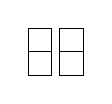
\begin{tikzpicture}
	\draw[] (0.3,-0.3) rectangle ++(0.3,0.3);
	\draw[] (0.3,0) rectangle ++(0.3,0.3);
	\draw[] (-0.1,0) rectangle ++(0.3,0.3);
	\draw[] (-0.1,-0.3) rectangle ++(0.3,0.3);
\end{tikzpicture}, but the former is not reliant on a specific ruleset. Rather, any combinatorial game has an instance equal to \gam{1}{}. However, the rules used to calculate the value of \Gm{=\gam{X}{Y}}, which are presented in the remaining of this section, help understand it better. The first practical rule in this text is finding the value of \gam{n}{} and \gam{}{{-}n}, for any natural number $n$.

Since 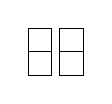
\begin{tikzpicture}
	\draw[] (0.3,-0.3) rectangle ++(0.3,0.3);
	\draw[] (0.3,0) rectangle ++(0.3,0.3);
	\draw[] (-0.1,0) rectangle ++(0.3,0.3);
	\draw[] (-0.1,-0.3) rectangle ++(0.3,0.3);
\end{tikzpicture} $= \gam{1}{}$, is it correct to assume that
$\underbrace{
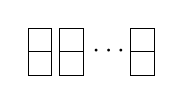
\begin{tikzpicture}
	\draw[] (1.2,-0.3) rectangle ++(0.3,0.3);
	\draw[] (1.2,0) rectangle ++(0.3,0.3);
	\draw[] (-0.1,0) rectangle ++(0.3,0.3);
	\draw[] (-0.1,-0.3) rectangle ++(0.3,0.3);
	\draw[] (0.3,0) rectangle ++(0.3,0.3);
	\draw[] (0.3,-0.3) rectangle ++(0.3,0.3);
	\node at (0.95, 0) {$\cdots$};
\end{tikzpicture}}_{n+1} = \gam{n}{}$? Yes, it is correct and the recursive nature of combinatorial games tell why. A $2\times 1$ board is equal to $1$ since Left has a move to spare. Therefore, two $2\times 1$ boards is equal to~$2$ since Left has a move to spare before reaching $1$. It is simple enough to visualize it in domineering boards. The fact is it should be simple to vizualise it in any combinatorial game. For any integer $k$, the game \gam{k}{} has the same value of the sum $\gam{k-1}{}+1$ if Left's best option $k$ is positive. If Left's best option is zero, then the game is equal to $1$, as already shown. If Left's best option is negative the result is zero, because Right cannot play, and  Left's move would result in the game $k$, which is negative, showing that whoever starts loses.  

In the case $k$ is positive, the addition $\gam{k-1}{} + 1$ was used. The notation is not the one used before, but it is possible replace $1$ with \gam{0}{}, as seen before. $\gam{k-1}{} + \gam{0}{}$ is an instance of addition described in the previous chapter. 

\begin{align*}
	\gam{k-1}{} + \gam{0}{} &\overset{def}{=} \gam{\gam{k-2}{} + \gam{0}{}, \gam{k-1}{} + \gam{}{}}{}\\
	&= \gam{\gam{k-2}{} + \gam{0}{}, \gam{k-1}{}}{}\\
	&\overset{def}{=} \gam{\gam{\gam{k-3}{} + \gam{0}{}}{}, \gam{\gam{k-2}{} + \gam{}{}}{}, \gam{\gam{k-2}{}}{}}{}\\
	&=\gam{\gam{\gam{k-3}{} + \gam{0}{}}{}, \gam{\gam{k-2}{}}{}, \gam{\gam{k-2}{}}{}}{}\\
	&=\gam{\gam{\gam{k-3}{} + \gam{0}{}}{}, \gam{\gam{k-2}{}}{}}{}\\
	&\overset{def}{\ldots}\\
	&=\underbrace{\{\{\ldots\{\{}_{k+1}\underbrace{\,|\,\}\,|\,\}\ldots\}\,|\,\}}_{k+1}\\
	&=\underbrace{\{\{\ldots\{\{}_{k} 0 \underbrace{\,|\,\}\,|\,\}\ldots\}\,|\,\}}_{k}\\
	&=\gam{k}{} = k + 1
\end{align*}

Every point discussed for \gam{X}{} is valid for \gam{}{Y}, through a similar argument. Up to this point, the integers and $\pm \frac{1}{2}$ are defined. The remaining numbers fall into three categories: the dyadic rationals - numbers of the form $\frac{a}{2^k}$, the numbers created in exactly infinite, $\aleph$, amount of steps, and the ones generated after more than infinite amount of steps. Of course the integers and $\frac{1}{2}$ fall into the first category.

In the case of $\Gm{} = \frac{1}{2} = \gam{0}{1}$, it is true that $G^L < G < G^R$. Is that always true? That is restricted for numbers, since in non-numbers \Gm{^R > G^L}. If Left makes a move from $G$ to $G^L$, is it true that Left has fewer spare moves in $G^L$ than in $G$? Before, as a side note, it was said that all possible RB-Hackenbush games are numbers, and the reason may help explain that it is true.

Suppose a game \Gm{ = \gam{X}{Y}} in which for all $x$ in $X$, $x$  is a number and for all $y$ in $Y$, $y$ is a number. Assume that $x_0$ in $X$ and $y_0$ in $Y$ are best moves for Left and Right respectively. If \Gm{} is not a number, than $x_0 \ge y_0$. Now consider \Hm an instance of RB-Hackenbush. A move in \Hm corresponds to removing a colored edge from a tree and all the edges that become disconnected to the floor. Assume again for \Hm that $x_0$ and $y_0$ are edges correspondent to the best moves for Left and Right respectively. That means that $x_0$ is similar to  
\begin{tikzpicture}
	\draw[blue, very thick] (0,0) -- (0,0.5);
	\node at (0, 0.9) {$\vdots$};
	\node at (-0.3, 0.9) {$\ddots$};
	\node at (0.3, 0.9) {\reflectbox{$\ddots$}};
\end{tikzpicture} and $y_0$ is similar to 
\begin{tikzpicture}
	\draw[red, dash pattern=on 3pt off 0.8pt, very thick] (0,0) -- (0,0.5);
	\node at (0, 0.9) {$\vdots$};
	\node at (-0.3, 0.9) {$\ddots$};
	\node at (0.3, 0.9) {\reflectbox{$\ddots$}};
\end{tikzpicture}. Is it possible that $G^{x_i} \ge G^{y_j}$?

Consider the game built by connecting $x_0$ to the floor. The game is definitely positive, as Left wins no matter who starts. If Right starts, he/she may have an available move in a edge above the one connected to the floor. Whether it is Left playing second or first, he/she may simply remove the blue edge connected to the floor, then Right has no moves remaining and loses the game. An analogous argument shows that $y_0$ in negative. Since $x_0$ is positive, the game $\Hm^{x_0}$ resulting from removing this positive branch is less positive, or more negative, than \Hm. The same way, $\Hm^{y_0}$ is more positive or less negative that \Hm. This fact, in turn, means that \Hm is a number.

Other phrasing for ``all RB-Hackenbush games are numbers" is ``it is not possible to make a move that improves your position in  RB-Hackenbush", or, ``Left cannot make a movement that increases the value of \Gm{}". Visualizing it brings the general idea why, in numbers, $G^L < G < G^R$. A more general approach is to consider, by induction, that $\Gm{^{LL}} < \Gm{^L} < \Gm{^{LR}}$ and $\Gm{^{RL}} < \Gm{^R} < \Gm{^{RR}}$. \Gm{^{LL}} translates to any possible Left move in \Gm{^L} and the others are defined similarly.

Consider the sum $\Gm{} - \Gm{^L}$. Before proceeding, the subtraction in this field means adding the negation. The negation of \gam{X}{Y} is \gam{-Y}{-X}. A good way to think of negation of a game \Gm{} as the same game \Gm{}, but with roles reversed. In the case of RB-Hackenbush for example, in ${-}\Gm{^L}$, Left plays the red edges. If Left starts, he/she can move to $\Gm{^L} - \Gm{^L} = 0$ and win the game. If Right starts, the game may be move to $\Gm{^R} - \Gm{^L}$ or $\Gm{} - \Gm{^{LR}}$. In the first case, it is clear that $\Gm{^R} - \Gm{^L} > 0$ because, from the definition of numbers, \Gm{^R} $>$ \Gm{^L}.
In the second case Left can move to $\Gm{^L} - \Gm{^{LR}}$, which is positive due to the induction hypothesis. Therefore, regardless who starts in $\Gm{} - \Gm{^L}$, Left wins, so the game is positive, meaning \Gm{>\Gm{^L}}. A similar argument shows that \Gm{<\Gm{^R}}.

Knowing this, however, is not enough to find the value of G. If $G = \{3 | 10\}$, it is clear that $3 < G < 10$ but what is the value of G? The simpler number that fits this interval, 4. What is called simpler is the minimal-birthday number that fits the interval. The word birthday comes from the initial analogy used to describe the creation of all the numbers. Before visiting the birthday tree and finishing explaining the simplicity principle, it is necessary to visit the definition of the comparison $\leq$.

Just like the definition of addition, the comparison is also done using game trees so it is the same for numbers and non-numbers. Consider the games \Gm{} and \Hm. \Gm{\leq \Hm} if they are equal or \Hm is more positive than \Gm{}. This condition is met if $\Hm > G^L$ and \Gm{<H^R}. These restrictions enforce that \Gm{=\gam{G^L}{G^R, H^R}} and $\Hm = \gam{G^L,H^L}{H^R}$, which guarantee the desired relation.

The birthday tree is the name given to the hierarchical structure that contains the definition of all surreal numbers. The tree is composed of layers, called generations, and each layer is a set of all the numbers formable with the available symbols. The zeroth generation is simply the set $\{0\} = \{\gam{}{}\}$. The first generation is the set $\{{-}1,0,1\}=$ \{\gam{}{0}, \gam{}{}, \gam{0}{}\}. The second is $\{-2,-1,\frac{-1}{2},0,\frac{1}{2},1,2\}$ and is equal to $\{\gam{}{{-}1},\gam{}{0},\gam{{-}1}{0},\gam{}{},\gam{0}{1}\gam{0}{},\gam{1}{}\}$. $0$ is called a zeroth generation number and $1$ and ${-}1$ are first generation numbers.

An important aspect of the generations is that, although labeling is not defined yet, they are fully ordered. Ordering is necessary for the simplicity rule because, as said before, \Gm{^L < \Gm{} < \Gm{^R}}. In order to find the value of \Gm{}, it is necessary to find a generation that contains both \Gm{^L} and \Gm{^R}, order it using the previously defined $\leq$ operation and find the oldest number lying strictly between \Gm{^L} and \Gm{^R}.

It is possible, however, to find cases where there are no numbers between \Gm{^L} and \Gm{^R}. In these case, one could look for a fitting number in the next generation. Another way to solve this is to notice that this cases occur if and only if both options are from the same generations and are neighbors in that generation. This condition implies that \Gm{^L = \frac{p}{2^q}} and \Gm{^R = \frac{p+1}{2^q}}. In this cases, the number in the next generation that lies strictly between them is the number \Gm{} and this number is labeled $\frac{2p + 1}{2^{q+1}}$.

The rules and definitions up until this point add up to:

\begin{center}
\Gm{ =} 
$
\begin{cases}
	0, &\text{if } G^L < 0 < G^R\\
	n+1, &\text{if } \Gm{= \gam{n}{}}\\
	-n-1, &\text{if } \Gm{= \gam{}{{-}n}}\\
	\frac{2p + 1}{2^{q+1}}, &\text{if } \Gm{= \gam{\frac{p}{2^q}}{ \frac{p+1}{2^q}}}\\
	\text{search the tree} &\text{otherwise}
\end{cases}
$
\end{center}

\vspace{0.6em}Some examples are $\frac{1}{4} =$ \gam{\frac{1}{10}}{\frac{3}{10}}, $\frac{1}{8} =$ \gam{0}{\frac{1}{4}}, $10 =$ \gam{9}{}, $1 =$ \gam{\frac{1}{2}}{}. The first and last examples require some manipulation as they would require a search on the birthday tree, as described previously. This would be a problem because both options of the first example would require an infinite number of generations to be created. However, since the embedded real numbers ought to be ordered the same and since surreals numbers are generated successively, the first number that fits the interval is the simplest that fits. Since $\frac{1}{10} < \frac{1}{4} < \frac{3}{10}$ and no older number older fits, the equality stands.

The remaining problematic example is $1 =$ \gam{\frac{1}{2}}{}. Consider the games, which happen to be numbers, \Gm{= \gam{0}{}} and $H = \gam{\frac{1}{2}}{}$. $G = 1$, directly from the simplicity rules. It is said that $H = 1$, but that is not a direct implication. It is possible, however, to show $G \leq H \leq G$. $H \leq G$, because $0.5$ is the only Left option of $H$, there are no Right options in $G$ and $0.5 < G = 1$. $G \leq H$, because $0$ is the only Left option of $G$, there are no Right options in $H$ and $0 < H$. The last inequality, $0 < H$, is true because in the game $H$, Left wins no matter who starts, and this means the game is positive.

It is possible to think of many other cases that require other manipulations to fall into the precisely defined rules. The reality is that the first four rules and the $\leq$ comparison are enough to label all the numbers. The fuzzy notion of simplicity brought in the last few paragraphs helps finding and understanding the reason for labels given but it is not necessary. The `Simplicity Rules' are actually just the first four rules.

\begin{center}
	\Gm{ =} 
	$
	\begin{cases}
		0, &\text{if } G^L < 0 < G^R\\
		n+1, &\text{if } \Gm{= \gam{n}{}}\\
		-n-1, &\text{if } \Gm{= \gam{}{{-}n}}\\
		\frac{2p + 1}{2^{q+1}}, &\text{if } \Gm{= \gam{\frac{p}{2^q}}{ \frac{p+1}{2^q}}}
	\end{cases}
	$
\end{center}

\subsection*{Numbers generated after infinite steps}

The formula above only allows \Gm{} to have an infinite amount of values, but the dimension of this infinity might not approach the stated in the beginning of the section yet. The remaining numbers are hidden in the end of infinite games. Infinite games, in this section, indicate board sizes that infinite, not infinite play, because, as explained before, this text only deals with short games. 

\begin{figure} [!ht]
\begin{center}
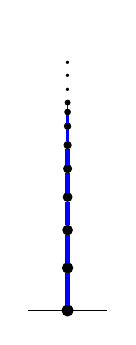
\begin{tikzpicture}
	\begin{scope} [every node/.style={scale=0.3, style=circle, draw, fill=black}]
		\node [scale=1.4] (1) at (0, -1.80){};
		\node [scale=1.3] (2) at (0, -1.26){};
		\node [scale=1.2] (3) at (0, -0.78){};
		\node [scale=1.1] (4) at (0, -0.36){};
		\node [scale=1]   (5) at (0, 0)      {};
		\node [scale=0.9] (6) at (0, 0.3)  {};
		\node [scale=0.8] (7) at (0, 0.54) {};
		\node [scale=0.7] (8) at (0, 0.72) {};
		\node [scale=0.6] (9) at (0, 0.84) {};
		\node [scale=0.2, fill=white, draw=none] at (0, 1.1) {$\vdots$};
	\end{scope}
	\draw (-0.5,-1.80) -- (0.5, -1.80);
	\draw[blue, ultra thick] (1)--(2);
	\draw[blue, ultra thick] (2)--(3);
	\draw[blue, ultra thick] (3)--(4);
	\draw[blue, ultra thick] (4)--(5);
	\draw[blue, ultra thick] (5)--(6);
	\draw[blue, thick] (6)--(7);
	\draw[blue, thick] (7)--(8);
	\draw[blue] (8)--(9);
	\node[scale=1.5] at (0, 1.3) {\scriptsize$\vdots$};
\end{tikzpicture}
\end{center}
\end{figure}

In the game above, Left has an infinite number of possible moves, but his/her move always leads to an integer. What is the value of this game? \gam{1,2,...}{}, the one more than the largest natural number. This number has been baptized much earlier in mathematics. It was called $\omega$, the first ordinal number, and the label is kept in the surreal numbers. It might not be as straight forward as finitely generated numbers, but the principle to calculate the value is the same.

For any finite number of red edges in \Gm{}, if you add the game above to \Gm{}, the result will be positive. However, it is also very simple to verify that $\omega$ is by far not the largest possible advantage. One simple  example for that is the following section.

$\omega$ is one of numbers generated in the $\aleph$ generation. Another is the number \gam{0}{\frac{1}{1}, \frac{1}{2}, \ldots}, labeled $\epsilon$. This number is positive, as Left wins no matter who starts, but it is smaller than any positive real number. A game with value $\epsilon$ may be simply the game of RB-Hackenbush starting with a blue edge and following with an infinite number of red edges.

These numbers are special in the sense that they are the first non-real numbers to show up, but they are not the only non-reals and they are not the only members of their generation. The integers and dyadic rationals show up in earlier generations, but the remaining reals all show up in the $\aleph$ generation. Chapter 5 will develop this topic a little further but, in general, it is not paramount to the topic of temperature.

\subsection*{Numbers generated after more than infinite steps}

\begin{figure} [!ht]
\begin{center}
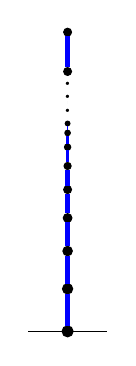
\begin{tikzpicture}
	\begin{scope} [every node/.style={scale=0.3, style=circle, draw, fill=black}]
		\node [scale=1.4] (1) at (0, -1.80){};
		\node [scale=1.3] (2) at (0, -1.26){};
		\node [scale=1.2] (3) at (0, -0.78){};
		\node [scale=1.1] (4) at (0, -0.36){};
		\node [scale=1]   (5) at (0, 0)      {};
		\node [scale=0.9] (6) at (0, 0.3)  {};
		\node [scale=0.8] (7) at (0, 0.54) {};
		\node [scale=0.7] (8) at (0, 0.72) {};
		\node [scale=0.6] (9) at (0, 0.84) {};
		\node [scale=0.2, fill=white, draw=none] at (0, 1.1) {$\vdots$};
		\node [scale=1] (10) at (0, 1.5) {};
		\node [scale=1] (11) at (0, 2) {};
	\end{scope}
	\draw (-0.5,-1.80) -- (0.5, -1.80);
	\draw[blue, ultra thick] (1)--(2);
	\draw[blue, ultra thick] (2)--(3);
	\draw[blue, ultra thick] (3)--(4);
	\draw[blue, ultra thick] (4)--(5);
	\draw[blue, ultra thick] (5)--(6);
	\draw[blue, thick] (6)--(7);
	\draw[blue, thick] (7)--(8);
	\draw[blue] (8)--(9);
	\node[scale=1.5] at (0, 1.3) {\scriptsize$\vdots$};
	\draw[blue, ultra thick] (10)--(11);
\end{tikzpicture}
\end{center}
\end{figure}

The game above is an infinite stack of blue edges with another one on the top. One could wrongly argue that this additional edge on the top is simply part of the infinite stack. This is a wrong argument because this additional edge on the top allows Left to move to $\omega$, and therefore, has the value of $\omega+1$, making the games different. The reason why in this case you can move to $\omega$ is that you can move on the top-most edge, while before, there was no top-most edge. This detail is paramount to understanding the statement found on the epigraph of this section.

A hypothetical John Horton Conway wrote the paragraph found on the epigraph near a cave close to the edge of the Indian Ocean, where a couple of future mathematicians went to find themselves. The words attributed to Conway by Knuth say that in the $\aleph$th day the universe appeared. That is because Knuth realizes that in that specific days all real numbers are generated.

However, again, accordingly to the hypothetical Conway, days kept passing by and more numbers were generated. The number $\omega+1$ is one of the infinitely many surreal numbers that are not real numbers. However, this is not the end of the story. In fact, even considering that $\omega + \omega + ...$ and $\omega^\omega$ are also generated in the same format, the important part might again be missed. That is because looking at large numbers is not the only way forward.

Now that $\epsilon$ is a known members of the $\aleph$ generation, it is possible to make numbers like \gam{0}{\epsilon} and \gam{-\epsilon}{0} and also games like \gam{1}{1 + \epsilon} and \gam{1-\epsilon}{1}. As the generations keep getting created it is easy to see that there are infinite numbers that are positive but less than any positive real number. In fact if taking the example around 1, it is possible to notice that between any two real numbers there are infinite non-real numbers. These non-real numbers are called infinitesimals.

There are still more non-real number that are not infinitesimals nor cardinals. A good example is the number $\sqrt{\omega} = \gam{1,2,3,\ldots}{\omega, \frac{\omega}{2},\frac{\omega}{4},\ldots}$. To verify that the label $\sqrt{\omega}$ is proper one would need to learn the definition of multiplication and verify that $\sqrt{\omega} \cdot \sqrt{\omega} = \omega$. As this text makes no use of multiplication this is not going to be verified. This example serves only to contribute to the point that there are truly many numbers originating from the simplicity rules.

\subsection*{The Surreal Numbers}

This text presents only few characteristics of the surreal numbers as they are not the focus. It is also not necessary to know every algebraic property of numbers to go forward with the study of temperature this text focus on. However, it so happens that with very few construction rules, the numbers contain all the reals, the ordinals, the infinitesimals numbers.

Because of its extremely simple definition and big expressiveness, it is an extremely interesting topic. The idea that the number of spare moves a player has might not be a real number might not be confusing, but it should be somewhat hard to accept. It is true that this fact is based on the construction Conway made and it is not necessarily true for all ways to analyze games, but the straight forward way of using game trees to build numbers lead to this characteristic.

Because the creation/discovery of surreals is very recent, it definitely makes people apprehensive as it is not clear if its properties are good or bad. The mathematician Phillip Ehrlich is an eloquent participant in this discussion. He makes the point that the surreals do not have an intrinsic problem and that they show an unifying nature between paths in mathematics. In one of his papers, Ehrlich proposes that, while the real numbers form, on his words, an arithmetic continuum, the surreals form the absolute arithmetic continuum\cite{7}.

However, it is still a problem converting the domain of typical studies, such as calculus, from the reals to the surreals. Integrals of functions in the surreals are particularly hard to define. In the 2015 revision of their paper \cite{8}, Salzedo and Swaminathan made important contributions. For reference, they proved the intermediate value theorem in \textbf{No}, how the class of all surreal numbers is called. However, for example, they used a definition of integration that, although solving a problem with previous definitions, they make it clear that other problems persist.

As the same authors point-out: ``The `Conway-Norton'\footnote{In ONAG 2nd edition page 228, Conway  tells that Norton's definition of integrals do not have desired properties.}
integral failed to have standard properties of real integration, however, such as translation
invariance: $\int_a^bf(x)dx = \int_{a-t}^{b-t}f(x+t)dx$, for any surreal function f and $a,b,t\in$ \textbf{No}. While Fornasiero fixed this issue \cite{9}, the new integral, like its predecessor, yields
$exp(\omega)$ instead of the desired $exp(\omega)-1$ for $\int_0^{\omega}exp(x)dx$". In the ``Open Questions" section of  the paper, the authors tell that there are still problems with their definition, meaning that the conversion of domains in integral studies is not completed, at least by 2015.

While many questions remain open, however, it is still possible to work with a subset of the surreals that only contain the reals for example. The remaining of the text does not require profound knowledge of anything that is not mentioned in regards to numbers.










    
% Data
    \chapter{Heating things up}
    
\definecolor{purple2}{RGB}{218,112,214}

This sections will provide new tools and ideas to analyze games and to do that, the same strategy of the previous section will be followed. Initially, the reader is presented with an intuitive idea and preliminary formulation of the problem. The first part contains many examples and its intent is to provide the reader enough to use the more mathematical heavy part to in fact gain advantage in any game played.

Now that enough is known about numbers, it is possible to work with non-numbers. The only known non-numbers at this point are the switches. But is knowing what they are enough to playing them? The game simpler cashing cheques will tell.

In this game there is a table with purple cheques. Each cheque has two numbers written on top, and, in each player's turn they will either pay one coin or cash a cheque that will grant him a number of coins equal to the correspondent associated integer. What is the best move for Left?

\begin{center}
\begin{tikzpicture}
	\node[draw] (title) at (0,1.5) {\textbf{Simpler Cashing Cheques}};
	\begin{scope} [every node/.style={style=circle, draw, fill=purple2}]
		\node at (-2,0) {8 $|$ 4};
		\node at (0,0) {5 $|$ 5};
		\node at (2,0) {1 $|$ 13};
	\end{scope}
\end{tikzpicture}
\end{center}

Definitely the move is not paying, as Left can earn money in his turn. A good thing to grasp from this example is that you should never play in a number, paying a coin in this case, if there are non-numbers, cashing a purple cheque in this case. Should Left cash 8, 5 or 1? 1, of course. The reader is encouraged to play as Left and trying to find the best possible outcome, but the answer is playing the hottest switch. Although the game above is not a switch, it is a sum of switches, and, because of that can benefit of the simplified notation discussed earlier.

\begin{align*}
	G =& \left(\frac{8-4}{2} \pm \frac{8+4}{2}\right) + \left(\frac{5-5}{2} \pm \frac{5+5}{2}\right) + \left(\frac{1-13}{2} \pm \frac{1+13}{2}\right) \\
	  =& (2 \pm 6) + (0 \pm 5) + (-6 \pm 7)\\
	  =& -4 \pm 7 \pm 6 \pm 5
\end{align*}

If you analyze the result above, it becomes clear that Left must play on the rightmost component as, although it will not provide many coins, it will prevent right from cashing a huge amount. It is very possible to build scenarios where a player would even pay for cashing a cheque if that prevented the opponent from getting rich. Now that playing a simpler cashing cheques became easy, a more challenging task will rise. How to play Domineering well?

Adding a number with a temperature in a simplified position, like the expression above, should be acceptable by anyone following up to this point. Following, in the other hand, numbers will be added together with non-numbers just like number are added together and this might cause confusion. However, understanding that this sum is possible and intuitive is simple.

Playing a sum of games is just like playing a game with a set of independent rulesets and components. \begin{center}
	\begin{tikzpicture}
		\node at (-0.5,0.1) {G =};
		\draw[] (0,0) rectangle ++(0.3,0.3);
		\draw[] (0.3,0) rectangle ++(0.3,0.3);
		\draw[] (0.6,0) rectangle ++(0.3,0.3);
		\node at (1.2,0.1) {$+$};
		\node[style=circle, draw, fill=purple2] at (2.1,0.1) {8 $|$ 4};
		\node at (3.1,0.1) {$+$};
		\draw[color=blue, ultra thick] (3.4, -0.1) -- (3.4, 0.5);
		\node[] at(3.6, -0.1) {,};
		\end{tikzpicture}
\end{center}
for example, is a game where each player makes a move\footnote{There are other ways of playing G that will not be discussed} in any of the components and loses if cannot make a move. In other words, \Gm{} is a game like every other, except for the more complex ruleset.

The result of this sum is obvious if all components are also numbers or switches. In the case of playing numbers and general non-numbers, sensible players will always play in non-numbers first. With this in mind other facts become clear. The first is that the temperature of a non-number added to a number is unaltered.

The second is that such a sum is actually a sum of non-numbers, added together with a number after they cool out. The sum of general non-numbers is thoroughly discussed in the remaining of the chapter, however, it worth noticing what the goal of this discussion is.

By the end of this section it will be thought how to convert any game in a 2D graphic composed of two \todo{curves} that collapse to one line at some point, whose axes is number x cooling factor. The purpose of all this is that if the ending point falls in the positive side, Left gets an advantage, and if it falls in the positive, right does.

To build this graphic one is required to traverse the game tree, so the effort may seem fruitless as the game tree itself provides the winning strategy by itself. However, in cases where the game tree resulting from the sum of games is too large or expensive for a computer to run, there is a good strategy to playing this sum without knowing the complete game tree. In order to build the thermograph and play the \defi{thermostrat}\footnote{This text will not present the thermostrat} correctly, there are a lot of minor concepts not discussed yet.

Other than the bias, playing a game like Domineering well involves the concepts of \defi{Left/Right stops}, \defi{toenail}, \defi{ambient temperature}, \defi{freezing point}, \defi{cooling}, \defi{heating} and a few others. To put all that together and provide a clear visualization of the best strategy, the thermograph.

\begin{center}
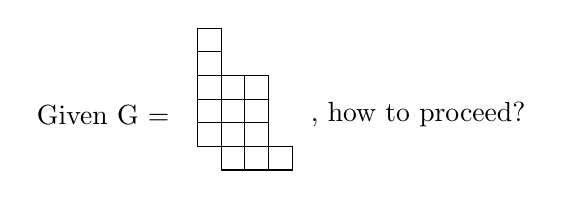
\begin{tikzpicture}
	\node at (-1.5,0.1) {Given G =};
	\draw[] (0,-0.6) rectangle ++(0.3,0.3);
	\draw[] (0.3,-0.6) rectangle ++(0.3,0.3);
	\draw[] (0.6,-0.6) rectangle ++(0.3,0.3);
	\draw[] (-0.3,-0.3) rectangle ++(0.3,0.3);
	\draw[] (0,-0.3) rectangle ++(0.3,0.3);
	\draw[] (0.3,-0.3) rectangle ++(0.3,0.3);
	\draw[] (-0.3,0) rectangle ++(0.3,0.3);
	\draw[] (0,0) rectangle ++(0.3,0.3);
	\draw[] (0.3,0) rectangle ++(0.3,0.3);
	\draw[] (-0.3,0.3) rectangle ++(0.3,0.3);
	\draw[] (0,0.3) rectangle ++(0.3,0.3);
	\draw[] (0.3,0.3) rectangle ++(0.3,0.3);
	\draw[] (-0.3,0.6) rectangle ++(0.3,0.3);
	\draw[] (-0.3,0.9) rectangle ++(0.3,0.3);
	\node at (2.5,0.1) {, how to proceed?};
\end{tikzpicture}
\end{center}

\begin{center}
	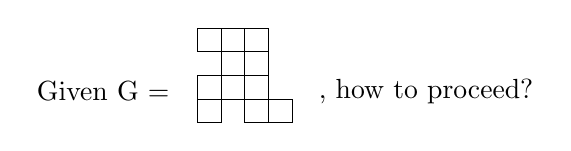
\begin{tikzpicture}
		\node at (-1.2,0.1) {Given G =};...
		\draw[] (0.6,-0.3) rectangle ++(0.3,0.3);
		\draw[] (0.9,-0.3) rectangle ++(0.3,0.3);
		\draw[] (0,-0.3) rectangle ++(0.3,0.3);
		\draw[] (0,0) rectangle ++(0.3,0.3);
		\draw[] (0.3,0) rectangle ++(0.3,0.3);
		\draw[] (0.6,0) rectangle ++(0.3,0.3);
		\draw[] (0.3,0.3) rectangle ++(0.3,0.3);
		\draw[] (0.6,0.3) rectangle ++(0.3,0.3);
		\draw[] (0,0.6) rectangle ++(0.3,0.3);
		\draw[] (0.3,0.6) rectangle ++(0.3,0.3);
		\draw[] (0.6,0.6) rectangle ++(0.3,0.3);
		\node at (2.9,0.1) {, how to proceed?};
	\end{tikzpicture}
\end{center}

G is definitely not a switch nor a sum of switches. It is possible to say the temperature in G is going to stay high for quite some time, because hotness is a term used to define the importance of the next move. A good place to start is writing out the game tree and building a temperature graphic of how it builds up from simpler positions until the more complicated ones.

To decrease the confusion that builds up in complicated positions, there is the idea of a cooling factor. The non-number \Gm{} cooled by $t$ degrees is represented by \Gm{_t} and is defined by:
\begin{center}
	\Gm{_t} = \gam{\Gm{^L_t} - t}{\Gm{^R_t} + t} $\forall t \leq t'$\\
	\Gm{_t} = x $\forall t > t'$\\
	Given $t'$ is the smallest cooling factor such\\
	that \Gm{_{t'}} is infinitesimally close to a number $x$,
\end{center}

The temperature $t(G)$ is equal to $t'$. Now that both axes are defined, some examples of thermographs:

\begin{tikzpicture}
	\begin{axis}
		[
		title = \Gm{=} \gam{3}{1},
		xmin=0.5,xmax=3.5, x dir=reverse, xtick={0, 1, 2, 3},
		ymax=3, ytick={0, 0.5, 1},
		axis x line*=none, axis y line*=none,
		axis line style={draw=none},
		y label style={rotate=-90,at={(current axis.north west)}, right=5mm},
		ylabel = \textbf{t}
		]
		\addplot[black] coordinates {
		(0.5,0)(3.5,0)
		};
		\addplot[black, very thick] coordinates {
		(0.9,-0.1)(2,1)
		};
		\addplot[black, very thick] coordinates {
		(3.1,-0.1)(2,1)
		};
		\addplot[black,-{Latex[length=3mm]}, very thick] coordinates {
		(2,1)(2,2)
	};
	\end{axis}
	\begin{axis}
	[
	at={(0.5\linewidth,0)},
	title = \Gm{=} \gam{0}{{-}4},
	xmin=-4.5,xmax=0.5, x dir=reverse, xtick={-4, -2, 0},
	ymax=3, ytick={0, 1, 2},
	axis x line*=none, axis y line*=none,
	axis line style={draw=none},
	y label style={rotate=-90,at={(current axis.north west)}, right=5mm},
	ylabel = \textbf{t}
	]
	\addplot[black] coordinates {
		(0.5,0)(-4.5,0)
	};
	\addplot[black, very thick] coordinates {
		(-0.1,-0.1)(-2,2)
	};
	\addplot[black, very thick] coordinates {
		(-4.1,-0.1)(-2,2)
	};
	\addplot[black,-{Latex[length=3mm]}, very thick] coordinates {
		(-2,2)(-2,2.5)
	};
	\end{axis}
	\begin{axis}
	[
	at={(0,-330)},
	title = \Gm{=} \gam{0}{0},
	xmin=-0.5,xmax=0.5, x dir=reverse, xtick={0},
	ymax=2, ytick={0, 1},
	axis x line*=none, axis y line*=none,
	axis line style={draw=none},
	y label style={rotate=-90,at={(current axis.north west)}, right=5mm},
	ylabel = \textbf{t}
	]
	\addplot[black] coordinates {
		(-0.5,0)(0.5,0)
	};
	\addplot[black, very thick] coordinates {
		(-0.1,-0.1)(0,0)
	};
	\addplot[black, very thick] coordinates {
		(0.1,-0.1)(0,0)
	};
	\addplot[black,-{Latex[length=3mm]}, very thick] coordinates {
		(0,0)(0,1.5)
	};
	\end{axis}
	\begin{axis}
	[
	at={(0.5\linewidth,-330)},
	title = \Gm{=} \gam{0}{\gam{0}{0}},
	xmin=-0.5,xmax=0.5, x dir=reverse, xtick={0},
	ymax=2, ytick={0, 1},
	axis x line*=none, axis y line*=none,
	axis line style={draw=none},
	y label style={rotate=-90,at={(current axis.north west)}, right=5mm},
	ylabel = \textbf{t}
	]
	\addplot[black] coordinates {
		(-0.5,0)(0.5,0)
	};
	\addplot[black, very thick] coordinates {
		(0,-0.1)(0,0)
	};
	\addplot[black, very thick] coordinates {
		(0.1,-0.1)(0,0)
	};
	\addplot[black,-{Latex[length=3mm]}, very thick] coordinates {
		(0,0)(0,1.5)
	};
	\end{axis}
\end{tikzpicture}


Some characteristics might be immediately apparent. The first is that the x-axis is reversed. The reason for that is to keep Right's movements to the right and Left's to the left. The second characteristic may be that all the thermographs end with a vertical \defi{mast}. The mast begins at $t'$ and indicates that \Gm{} is a number from that point forward. The last one is that the graphic continues past the $y=0$ line. It is worth noticing that the difference between the last two thermographs is below the $y=0$ line.

Toenails, the segments below the $y=0$ line, are important and may seem different, but they are actually simple extensions of the graphic. The reason for the last two toenails to be different is that cooling is applied to all the Left and Right alternatives, but in opposite directions. It is important to remember \hbox{\Gm{_t} = \gam{\Gm{^L_t} - t}{\Gm{^R_t} + t}}, because it explains the difference. Both Left's and the first Right's toenail came from cooling 0, but the second Right's toenail came from cooling \gam{0}{0}.

The next example, the second of non-switch hot games, shows how cooling $L$ and $R$ alternatives work.\\

\begin{figure}[H]
\begin{center}
	\scalebox{0.8}{
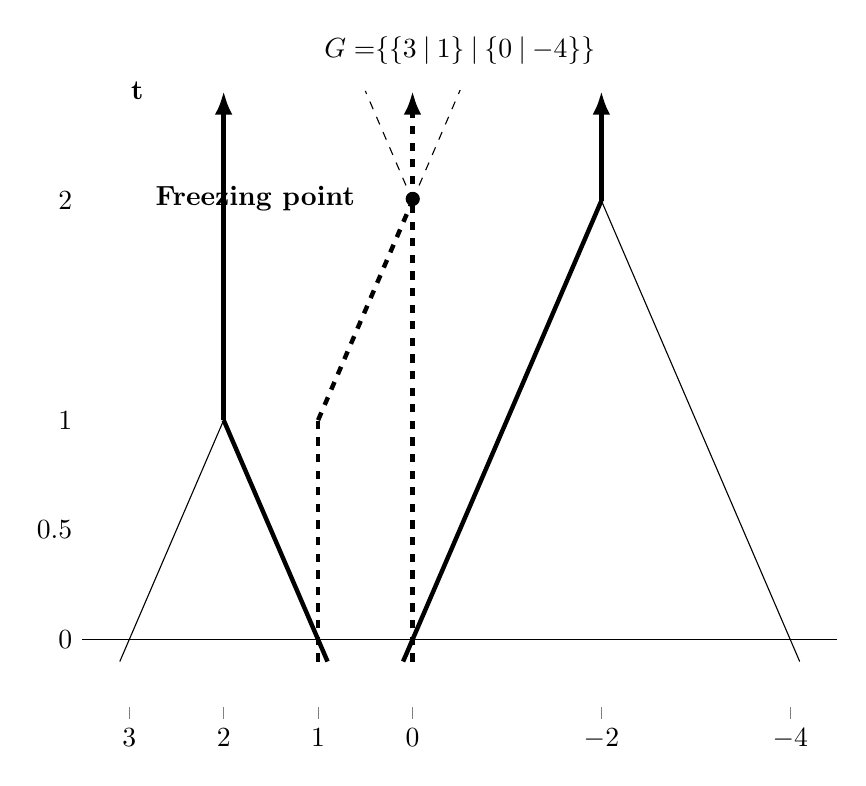
\begin{tikzpicture}
	\node[] at (2.2, 6.6) {\textbf{Freezing point}};
	\node[scale=0.5, circle, draw, fill=black] at (4.2, 6.6) {};
	\begin{axis}
		[
		title = \Gm{=}\gam{\gam{3}{1}}{\gam{0}{{-}4}},
		xmin=-4.5,xmax=3.5, x dir=reverse, xtick={-2, -4, 0, 1, 2, 3},
		ymax=2.5, ytick={0, 0.5, 1, 2},
		axis x line*=none, axis y line*=none,
		axis line style={draw=none},
		y label style={rotate=-90,at={(current axis.north west)}, right=5mm},
		ylabel = \textbf{t},
		scale=1.4
		]
		
		\addplot[black] coordinates {
			(-4.5,0)(3.5,0)
		};
		\addplot[ultra thick] coordinates {
			(0.9,-0.1)(2,1)
		};
		\addplot[black] coordinates {
			(3.1,-0.1)(2,1)
		};
		\addplot[-{Latex[length=3mm]}, ultra thick] coordinates {
			(2,1)(2,2.5)
		};
		\addplot[ultra thick] coordinates {
			(0.1,-0.1)(-2,2)
		};
		\addplot[] coordinates {
			(-4.1,-0.1)(-2,2)
		};
		\addplot[-{Latex[length=3mm]}, ultra thick] coordinates {
			(-2,2)(-2,2.5)
		};
		\addplot[black, dashed, ultra thick] coordinates {
			(1,-0.1)(1,1)
		};
		\addplot[black, dashed, ultra thick] coordinates {
			(0,-0.1)(0,2)
		};
		\addplot[black, dashed, ultra thick] coordinates {
			(1,1)(0,2)
		};
		\addplot[black, dashed] coordinates {
			(0,2)(-1,3)
		};
		\addplot[black, dashed] coordinates {
			(0,2)(0.5,2.5)
		};
		\addplot[black, dashed, ultra thick, -{Latex[length=3mm]}] coordinates {
			(0,2)(0,2.5)
		};
	\end{axis}
\end{tikzpicture}}
\end{center}
\caption{The dissection of a thermograph}
\end{figure}



In the example above, the thick dashed thermograph is the thermograph of G. The light dashed segments are illustrative extensions of the cooling of L and R. The bold lines were used to show what part of L and R are taken into consideration: Right's slant is used to build Left's slant and vice-versa. The reason for this is that after either player makes a move, it will be the opponent's turn to move, and, this way, the opposing slant is the important one.

It is also worth mentioning that a freezing point will always be reached after an equal amount of move by each player. In the example above, the freezing point is the same as the junction point where the right slant bends, but that is not always the case. Before visiting \todo{siegel}'s formulation of the problem, one that brings good notation and formalism, an example of a real scenario is due. In a fun game each player has more than one option for their moves and that has not been addressed yet.

What is the thermograph of the game \Gm{=}
	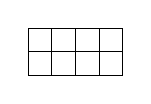
\begin{tikzpicture}
		\draw[] (0.6,-0.6) rectangle ++(0.3,0.3);
		\draw[] (0.3,-0.6) rectangle ++(0.3,0.3);
		\draw[] (0.9,-0.6) rectangle ++(0.3,0.3);
		\draw[] (0,-0.6) rectangle ++(0.3,0.3);
		\draw[] (0,-0.3) rectangle ++(0.3,0.3);
		\draw[] (0.3,-0.3) rectangle ++(0.3,0.3);
		\draw[] (0.6,-0.3) rectangle ++(0.3,0.3);
		\draw[] (0.9,-0.3) rectangle ++(0.3,0.3);
	\end{tikzpicture} ? 

\begin{figure} [!ht]
\begin{center}
\begin{tikzpicture}
	[
	sibling distance=150pt,
	level distance=100pt,
	level 1/.style={sibling distance=4cm},
	level 2/.style={sibling distance=1.7cm},
	every node/.style = {
	},
	every child/.style = {
		ultra thick
	}
	]

\node[draw] (title) at (0, 1) {Game Tree};

\node {
	\begin{tikzpicture}
		\draw[] (0.6,-0.6) rectangle ++(0.3,0.3);
		\draw[] (0.3,-0.6) rectangle ++(0.3,0.3);
		\draw[] (0.9,-0.6) rectangle ++(0.3,0.3);
		\draw[] (0,-0.6) rectangle ++(0.3,0.3);
		\draw[] (0,-0.3) rectangle ++(0.3,0.3);
		\draw[] (0.3,-0.3) rectangle ++(0.3,0.3);
		\draw[] (0.6,-0.3) rectangle ++(0.3,0.3);
		\draw[] (0.9,-0.3) rectangle ++(0.3,0.3);
	\end{tikzpicture}}
child[blue, level distance=80pt] {node[black] {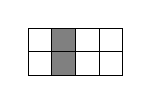
\begin{tikzpicture}
			\draw[] (0.6,-0.6) rectangle ++(0.3,0.3);
			\draw[fill=gray] (0.3,-0.6) rectangle ++(0.3,0.3);
			\draw[] (0.9,-0.6) rectangle ++(0.3,0.3);
			\draw[] (0,-0.6) rectangle ++(0.3,0.3);
			\draw[] (0,-0.3) rectangle ++(0.3,0.3);
			\draw[fill=gray] (0.3,-0.3) rectangle ++(0.3,0.3);
			\draw[] (0.6,-0.3) rectangle ++(0.3,0.3);
			\draw[] (0.9,-0.3) rectangle ++(0.3,0.3);
	\end{tikzpicture}}
	child[blue] {node[black] {\gam{1}{}}}
	child[blue] {node[black] {\gam{1}{{-}1}}}
	child[red, dashed] {node[black] {\gam{{-}1}{1}}}
}
child[blue] {node[black] {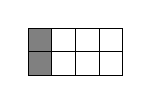
\begin{tikzpicture}
			\draw[] (0.6,-0.6) rectangle ++(0.3,0.3);
			\draw[] (0.3,-0.6) rectangle ++(0.3,0.3);
			\draw[] (0.9,-0.6) rectangle ++(0.3,0.3);
			\draw[fill=gray] (0,-0.6) rectangle ++(0.3,0.3);
			\draw[fill=gray] (0,-0.3) rectangle ++(0.3,0.3);
			\draw[] (0.3,-0.3) rectangle ++(0.3,0.3);
			\draw[] (0.6,-0.3) rectangle ++(0.3,0.3);
			\draw[] (0.9,-0.3) rectangle ++(0.3,0.3);
	\end{tikzpicture}}
	child[blue] {node[black] {\gam{1}{}}}
	child[blue] {node[black] {\gam{1}{{-}1}}}
	child[red, dashed] {node[black] {\gam{{-}1}{0,1}}}
}
child[red, dashed, level distance=80pt] {node[black, solid] { 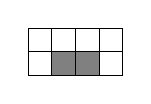
\begin{tikzpicture}
			\draw[fill=gray] (0.6,-0.6) rectangle ++(0.3,0.3);
			\draw[fill=gray] (0.3,-0.6) rectangle ++(0.3,0.3);
			\draw[] (0.9,-0.6) rectangle ++(0.3,0.3);
			\draw[] (0,-0.6) rectangle ++(0.3,0.3);
			\draw[] (0,-0.3) rectangle ++(0.3,0.3);
			\draw[] (0.3,-0.3) rectangle ++(0.3,0.3);
			\draw[] (0.6,-0.3) rectangle ++(0.3,0.3);
			\draw[] (0.9,-0.3) rectangle ++(0.3,0.3);
	\end{tikzpicture}}
	child[blue, solid] {node[black] {\gam{{-}1}{0, 1}}}
	child[red] {node[black] {\gam{1}{}}}
	child[red] {node[black] {\gam{0}{0}}}
}
child[red, dashed] {
	node[black, solid] { 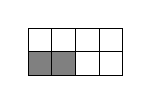
\begin{tikzpicture}
	\draw[] (0.6,-0.6) rectangle ++(0.3,0.3);
	\draw[fill=gray] (0.3,-0.6) rectangle ++(0.3,0.3);
	\draw[] (0.9,-0.6) rectangle ++(0.3,0.3);
	\draw[fill=gray] (0,-0.6) rectangle ++(0.3,0.3);
	\draw[] (0,-0.3) rectangle ++(0.3,0.3);
	\draw[] (0.3,-0.3) rectangle ++(0.3,0.3);
	\draw[] (0.6,-0.3) rectangle ++(0.3,0.3);
	\draw[] (0.9,-0.3) rectangle ++(0.3,0.3);
	\end{tikzpicture}}
		child[blue, solid] {node[black] {\gam{{-}1}{1}}}
		child[blue, solid] {node[black] {\gam{{-}1}{0,1}}}
		child[red] {node[black] {\gam{}{{-}1}}}
	}
;

\end{tikzpicture}
\end{center}
\end{figure}

\hspace{-1cm}
\begin{tikzpicture}
\begin{axis}
	[
		title = \gam{\gam{1}{{-}1},2}{0},
		xmin=-1.5,xmax=2.5, x dir=reverse, xtick={-1,0, 1, 2},
		ymax=2, ytick={0, 1, 1},
		scale=0.5,
		style thermograph
	]
	\addplot[] coordinates {(3.5,0)(-1.5,0)};
	\addplot[-{Latex[length=3mm]}] coordinates { (2,-0.1)(2,1.5)};
	\addplot[-{Latex[length=3mm]}] coordinates { (0,-0.1)(0,1.5)};
	\addplot[ultra thick] coordinates { (-0.1,-0.1)(1,1)};
	\addplot[ultra thick] coordinates { (2.1,-0.1)(1,1)};
	\addplot[-{Latex[length=3mm]}, ultra thick] coordinates { (1,1)(1,1.9)};
	\addplot[] coordinates {(1.1,-0.1)(0,1)};
	\addplot[red, densely dashed] coordinates {(-1.1,-0.1)(0,1)};
\end{axis}
\begin{axis}
	[
	title = \gam{2,\gam{1}{{-}1}}{{-}\frac{1}{2}},
	xmin=-1.5,xmax=2.5, x dir=reverse, xtick={-0.5, 1.25,2},
	ymax=2.3, ytick={0, 1.25},
	scale=0.5,
	at={(4cm,0)},
	style thermograph
	]
	\addplot[] coordinates {(2.5,0)(-1.5,0)};
	\addplot[-{Latex[length=3mm]}] coordinates { (2,-0.1)(2,1.5)};
	\addplot[-{Latex[length=3mm]}] coordinates { (-0.5,-0.1)(-0.5,1.5)};
	\addplot[ultra thick] coordinates { (-0.6,-0.1)(0.75,1.25)};
	\addplot[ultra thick] coordinates { (2.1,-0.1)(0.75,1.25)};
	\addplot[-{Latex[length=3mm]}, ultra thick] coordinates { (0.75,1.25)(0.75,2.2)};
	\addplot[] coordinates {(1.1,-0.1)(0,1)};
	\addplot[red, densely dashed] coordinates {(-1.1,-0.1)(0,1)};
	\addplot[-{Latex[length=3mm]}] coordinates { (0,1)(0,1.5)};
\end{axis}
\node[] at (9.3,2) {\gam{{-}\frac{1}{2}}{2, \gam{0}{0}}};
\node[] at (9.3,1.5) {$=0$};
\begin{axis}
	[
	title = \gam{{-}\frac{1}{2}, 0}{{-}2},
	xmin=-2.5,xmax=0.5, x dir=reverse, xtick={-2,-1,0},
	ymax=2.5, ytick={0, 1, 1.75},
	scale=0.5,
	at={(12cm,0)},
	style thermograph
	]
	\addplot[] coordinates {(-3.5,0)(1.5,0)};
	\addplot[-{Latex[length=3mm]}] coordinates { (0,-0.1)(0,1.5)};
	\addplot[-{Latex[length=3mm]}] coordinates { (-0.5,-0.1)(-0.5,1.5)};
	\addplot[-{Latex[length=3mm]}] coordinates { (-2,-0.1)(-2,1.5)};
	\addplot[ultra thick] coordinates {(0.1,-0.1)(-1,1)};
	\addplot[ultra thick] coordinates { (-2.1,-0.1)(-1,1)};
	\addplot[-{Latex[length=3mm]}, ultra thick] coordinates { (-1,1)(-1,1.75)};
\end{axis}
\end{tikzpicture}

\hspace{-2.3cm}
\begin{tikzpicture}
\begin{axis}
	[
	title = \Gm{},
	xmin=-2.5,xmax=2.5, x dir=reverse, xtick={-2,-1,0,1,2},
	ymax=2.5, ytick={0, 1, 1.75},
	scale=1,
	at={(0,-7.5cm)},
	style thermograph
	]
	\addplot[] coordinates {(-2.5,0)(2.5,0)};
	\addplot[] coordinates {(0.1,-0.1)(-1,1)};
	\addplot[] coordinates { (-2.1,-0.1)(-1,1)};
	\addplot[] coordinates { (2.1,-0.1)(0.75,1.25)};
	\addplot[] coordinates { (2.1,-0.1)(1,1)};
	\addplot[] coordinates { (1,1)(-0.1,-0.1)};
	\addplot[] coordinates { (0.75,1.25)(-0.6,-0.1)};
	\addplot[-{Latex[length=3mm]}] coordinates { (-1,1)(-1,1.75)};
	\addplot[-{Latex[length=3mm]}] coordinates { (0,-0.1)(0,1.5)};
	\addplot[-{Latex[length=3mm]}] coordinates { (0.75,1.25)(0.75,2.3)};
	\addplot[-{Latex[length=3mm]}] coordinates { (1,1)(1,2.3)};
\end{axis}
\node[] at (7.5,-5) {$\underset{\text{Removing  dominated moves}}{\Rightarrow}$};
\begin{axis}
	[
	title = \Gm{},
	xmin=-0.5,xmax=2.5, x dir=reverse, xtick={2,1,0},
	ymax=2.5, ytick={0, 1, 1.75},
	scale=1,
	at={(0.5*\linewidth + 2cm,-7.5cm)},
	style thermograph
	]
	\addplot[] coordinates {(-2.5,0)(2.5,0)};
	\addplot[] coordinates { (2.1,-0.1)(1,1)};
	\addplot[] coordinates { (1,1)(-0.1,-0.1)};
	\addplot[] coordinates { (-0.1,-0.1)(0,0)};
	\addplot[-{Latex[length=3mm]}] coordinates { (0,-0.1)(0,1.5)};
	\addplot[-{Latex[length=3mm]}] coordinates { (1,1)(1,2.3)};
\end{axis}
\end{tikzpicture}
\begin{center}
\begin{tikzpicture}
\begin{axis}
	[
	title = \Gm{},
	xmin=-1.5,xmax=1.5, x dir=reverse, xtick={1,0,-1},
	ymax=2.5, ytick={1},
	scale=1,
	at={(0.5*\linewidth + 1cm,-10)},
	style thermograph
	]
	\addplot[] coordinates {(-1.5,0)(1.5,0)};
	\addplot[ultra thick] coordinates { (-0.1,-0.1)(0,0)};
	\addplot[-{Latex[length=3mm]}, ultra thick] coordinates { (0,-0.1)(0,1.5)};
\end{axis}
\end{tikzpicture}
\end{center}

The thermograph of \Gm{} and \gam{\gam{0}{0}}{0} are the same, although they are different games. From the steps taken to build that thermograph one can see that not all available moves contribute to build the temperature. Because we can calculate that some moves are strictly worse than others it makes sense that they should be ignored, but the thermograph shows exactly why.

When Left moves, he/she should avoid giving Right greater advantage over getting him/herself a possible better outcome. In the first thermograph, it is clear that $2$ is greater, meaning it is more positive, or better for Left, than \gam{1}{{-}1} The reason for that is because the red right slant is more to the right than $2$, not because the left slant is more to the right than $2$.

The comment that \Gm{}'s thermograph is the same as that of the game \gam{\gam{0}{0}}{0}, but they are different games is surprisingly paramount to playing games well. It is so important that games of the form \gam{\gam{x}{0}}{0}$=-_x$ and \gam{0}{\gam{0}{{-x}}}$=+_x$ receive special names, minies an tinies, respectively. The game above is negative, of course, but Right's advantage really small.

In the game above, \Gm{=-_2}, Right's advantage is much smaller than that of $-_1$. In fact, for any number $x,y | x > y \ge 0$, any multiple of $-_x$ is less negative than $-_y$. It may come of as a surprise because usually multiplication is only made between numbers, but, in fact, this observation makes sense when a real example is provided.

One should think of minies and tinies as late fees. In the case of tinies, if Left makes a move, he/she is fine. However, if he/she does not, Right may send a warning e-mail that tells Left to do so. If, after the e-mail, Left makes the move, he/she is fine again, but if Left does not, Right can charge a late fee from Left.

The reason for any multiple of $+_x$ remain smaller than $+_y$ is just that. Since there is the warning phase in the game, players will always be in time to reply. The only case where a reply is not worth is when there are more important moves to make. Because, the only factor, in this case, that makes a move more or less worth is the value of x, it does not matter how many $+_x$ there are. When playing situations where one can choose between quantity of minies/tinies over quality, the choice for quality is always the correct one.

One important situation, however, did not happen in the game above. There will be cases where there is no clear best move for a component $C$, and that will depend on the ambient temperature of the game. The reader can see that if \Gm{=C}, then there are best first move to make. In the example above, \Gm{^L = \gam{2}{0}} and \Gm{^R = 0}.

However, if other components are added together with $C$, the best first move in $C$ may change. The reader can imagine the situation where it Left turn to play, but Right has an important move to make next. Knowing that, Left makes a greedy move, that allows the opponent to acquire more advantage than other options, but allows him/herself more advantages if Right does not capitalize. Right is cornered between making the previous important move and this new option Left allowed.

For example, check the following game of extended simpler cashing cheques, where the previous rules apply, but the players may also play on yellow squares. The yellow squares allows players to select any purple correspondent purple cheque before disappearing. Purple cheques might also show negative values, indicating the opponent receives the promised coins.

\begin{figure}[H]
\begin{center}
	\scalebox{0.9}{
	\begin{tikzpicture}
		\node[draw] (title) at (3,1.5) {\textbf{Extended Simpler Cashing Cheques}};
		\begin{scope} []
			\draw[fill=yellow] (-1,-1) rectangle ++(8,1.9);
			\draw[fill=yellow] (0,-3) rectangle ++(6,1.9);
			\draw[fill=yellow] (0,-5) rectangle ++(6,1.9);
			\node[] at (-2,0) {\Large A};
			\node[] at (-1,-2) {\Large B};
			\node[] at (-1,-4) {\Large C};
			\node[circle, draw, fill=purple2] at (0,0) {7 $|$ {-}9};
			\node[circle, draw, fill=purple2] at (2,0) {28 $|$ {-}4};
			\draw[thick] (3,-0.75) -- (3,0.75);
			\node[circle, draw, fill=purple2] at (4,0) {{-}3 $|$ 1};
			\node[circle, draw, fill=purple2] at (6,0) {2 $|$ 22};
			\node[circle, draw, fill=purple2] at (1,-2) {{-}4 $|$ 2};
			\node[circle, draw, fill=purple2] at (3,-2) {9 $|$ 5};
			\draw[thick] (4,-2.75) -- (4,-1.25);
			\node[circle, draw, fill=purple2, scale=0.9] at (5,-2) {{-}11 $|$ {25}};
			\node[circle, draw, fill=purple2, scale=0.95] at (1,-4) {{-13} $|$ 11};
			\draw[thick] (2,-4.75) -- (2,-3.25);
			\node[circle, draw, fill=purple2, scale=0.94] at (3,-4) {{-}25 $|$ 23};
			\node[circle, draw, fill=purple2] at (5,-4) {{-}19 $|$ 35};
		\end{scope}
	\end{tikzpicture}
}
\end{center}
\caption{Sum of hot components without dominated moves}
\end{figure}

It is a good thing now to consider the game above as the sum of three components, $A,B,C$ from top to bottom. It is completely clear what the best moves for left and right are in each of the components. However, from the thermograph of the components, one will find that no moves are dominated, they all influence the resulting thermograph. As seen before, this mean that depending on the ambient temperature the best move in each component will vary.

In the last example, the best move for Left is actually to play in $B$ and make the move to \gam{9}{{-}5}. In this case, the reader should notice that $A + B - 5$ is less negative than the original game, but also that Right will not necessarily move in \gam{9}{{-}5}. Left's move, is an example of taking advantage of the fact the opponent will be distracted moving elsewhere to make the best of, in this case, a bad situation.













    
% Methods
    \chapter{Methods}
    \textcolor{red}{In this Chapter, you present in more concrete terms the method(s) you are going to apply. And as always in research, it is good to demonstrate awareness of the weaknesses or limitations of the method you use. It makes no difference if you work with interviews, econometric models, or a comprehensive analysis of data from various sources. Transparency should be the guideline: make it possible for your readers to follow, or even repeat, your analysis!}

\section{The Approach [or Model]}
Lorem ipsum dolor sit amet, consectetur adipiscing elit. Duis ut ipsum nec orci interdum sollicitudin ut eu nunc. Pellentesque ultricies eros in justo sagittis, eget blandit velit aliquet. Aenean ac lectus nibh. Quisque ac est pellentesque, ullamcorper sem sit amet, pharetra quam. Morbi ullamcorper placerat diam, sed tincidunt odio.
    
% Empirical Analysis
    \chapter{Empirical Analysis}
    \textcolor{red}{This chapter covers three areas: analysis of the data; discussion of the results of the analysis; and how your findings relate to the literature. The analysis of the data can be discussed here but the details of any analysis, such as statistical calculations, should be shown in the appendices. You should present any discussion clearly and logically and it should be relevant to your research questions/hypotheses or aims and objectives. Insert any tables or figures that you decide are important in a relevant part of the text not in the appendices, and discuss them fully. Make sure that you relate the findings of your primary research to your literature review. You can do this by comparison: discussing similarities and particularly differences. If you think your findings have confirmed some literature findings, say so and say why. If you think your findings are at variance with the literature, say so and say why.}
\section{Results}
Lorem ipsum dolor sit amet, consectetur adipiscing elit. Duis ut ipsum nec orci interdum sollicitudin ut eu nunc. Pellentesque ultricies eros in justo sagittis, eget blandit velit aliquet. Aenean ac lectus nibh. Quisque ac est pellentesque, ullamcorper sem sit amet, pharetra quam. Morbi ullamcorper placerat diam, sed tincidunt odio.

\textcolor{red}{When placing tables (\autoref{tab:econ}) within the body of the text, the citation is placed above the table.} 


\vfill

\newpage 

\section{Discussion}
Lorem ipsum dolor sit amet, consectetur adipiscing elit. Duis ut ipsum nec orci interdum sollicitudin ut eu nunc. Pellentesque ultricies eros in justo sagittis, eget blandit velit aliquet. Aenean ac lectus nibh. Quisque ac est pellentesque, ullamcorper sem sit amet, pharetra quam. Morbi ullamcorper placerat diam, sed tincidunt odio.

\textcolor{red}{When placing figures (illustrations, pictures, graphs, diagrams, charts, maps etc.) within the body of the text, the citation is placed below the figure (\autoref{fig:moun})}


    
% Conclusion
    \chapter{Conclusion}
    Combinatorial game theory is a new field in mathematics that was initially found in the blend of recreational mathematics, combinatorics and number theory. While the initial focus is finding strategies to play better and win games, the developments it prompted in other areas of mathematics have their own place, independent of the initial purpose. The Surreal Numbers form a class with many interesting properties and found much enthusiasm for that reason, not because it was necessary to analyze games.

However, the surreal numbers inevitably carry the simplicity inherited from the mathematical plays it was created/discovered for. It is commonplace to learn how to breach the gap between rational and real numbers only in superior education, partially because any of the common constructions involves operations and procedures not used in school. Surreal Numbers give for free the construction of real numbers from its few and simple rules. Not only the reals, but a definition of positivity and negativity that dismisses comparison, a common method for the creation of all the numbers, new numbers and, at last, a direct way of visualizing each number with RB-Hackenbush games. Numbers are the main building block the text used to analyze games.

The non-numbers, a name used in this text for games with temperatures, are the remaining games and required more elements and concepts to be understood. The thermograph, or the form commonly used to visualize temperature, options, stops and boiling points, is extensively analyzed and the text presents one of the most recent related results.

The reader that understands all the featured topics and is able to replicate calculations and results to games other than the mentioned might carry the false belief that understands all of combinatorial game theory. This text, however, only describes the class of partisan games leaving many variations even unmentioned. Not only the focus is specific, but also not all perspectives necessary to tackle the problem of finding the best move are visited.

These information serves to show that there is much more to the field, not that little progress understanding it was made. In fact, it is fair to state that the classes of games discussed in the text are the more complicated ones and many of the definitions apply to other classes.

Both in the results discussed and the ones omitted there is a common trend in this field. The definitions are always simple, but powerful enough to allow many questions, and, although there are many open questions, the proofs are and solutions are simple as well. The procedure to build all dyadic rationals in domineering boards, for example, is based on a theorem provable in two lines of text and applying it is the simplest of ways. Although its explanation is simple, it remained open for years and the resulting pattern is not something that would be found before the proof.

Finding the upper bound to temperature is another case where the question remained open for long, but the strategy used to answer is simplicity: it consists only of listing and manipulating properties of the thermographs.That is not to say that the bounding of temperature is completely solved but the progress made used simple steps.

From this perspective combinatorial game theory is a beautiful field in mathematics. The definitions it is based upon are extremely few in number and very simple in form, but they allow proving more complex problems in a uncomplicated manner. However, in this text, one of the unvisited places in the field is computational complexity. In practice, calculating values is not an easy problem.

The other featured aspect skipped is the variety of forms combinatorial games might take, because the text only deals with partisan games played on normal conditions. The remaining contains a brief description of these two skipped problems and points toward texts on th respective subjects. This chapter, that finalizes the text, also addresses a few of the next steps studying or researching the field and ends with a personal reflection on the learning, implementing and writing experiences involved in this work.


\subsection*{Undeveloped Pieces}

\subsubsection*{Complexity}

The text repeatedly made the case that most concepts are simple in Combinatorial Game Theory. It said, for example, that the method used to find the number a game is equal to is straight-forward. However this hides an important factor.

Either calculating the number or building a thermograph requires, first, traversing the game tree. Traversing this tree and calculating the values is simple enough, but it is slow. And it is slow because this tree quickly becomes large. For example, consider the following game of Domineering.

\begin{center}

\begin{tikzpicture}
\draw[step=0.5cm,color=gray] (-1,-1) grid (1,1);
\newcounter{mycount}
\setcounter{mycount}{`A}
\foreach \y in {+0.75,+0.25,-0.25,-0.75}
\foreach \x in {-0.75,-0.25,0.25,0.75}
\node at (\x,\y) {\addtocounter{mycount}{1}};
\end{tikzpicture}
\end{center}

There are, of course, 25 squares, which means that at most 12 moves might be made and in addition, some of these moves might be equivalent, so they do not have to be computed multiple times. It happens that only 604 nodes, or different position, may be reached\cite{1}. In a $6\times 6$ board it jumps to $17,232$ and in $7\times 7$ and $8\times 8$ board it goes to $408,260$ and $441,990,070$ nodes. Although these results are from 1998, results on larger boards took many years and only in 2016 a result for $11 \times 11$\cite{2} board was found, but abandoning a naive building of a game tree. The game tree of a $9\times 9$ board has around 25 trillion nodes.

If not clear at first it should be now that there is no known form of calculating values for games in polynomial time is respect to their sizes. The question, then, is in what class of problems it fits. It happens that many of the games are known to be PSPACE-complete and some are known to be EXPTIME.

There is of course much more to be said an it is another very interesting topic. A good starting point is \textit{Playing Games with Algorithms: Algorithmic Combinatorial Game Theory}\cite{3}. The thesis \textit{Games, Puzzles, and Computation} is more extensive, covering different classes of games, but may be more complex. Regardless of the suggested texts, there is a large amount of great books on complexity theory.

\subsubsection*{Other games}

By looking at the definition of combinatorial games given in the beginning of section 2, it is easy to come up with games that do not fit well the class of games studied, the short games. One clear example is the game of chess, because there are ties and there are drawn positions.

However, games like chess are not the only class of games that behave differently. Consider G-Hackenbush, a variation of RB-Hackenbush, in which both blue and red edges are replaced by green ones. Green edges may be removed by either player, meaning that both players have the same available moves regardless of the position. The class of games that follow this property is called Impartial Games.

Impartial games were the first games studied, previously to the consolidation of the modern form of the field. They have an interesting property of being reducible to an instance of a game of Nim. 

Games like chess, on the other hand, are not so simple. there are more classes of results than short games, which allows games to become more complex. Such games benefit from knowing short game's theory but do require further concepts. A good place to start is the corresponding chapter in the book \textit{Combinatorial Game Theory}.


\subsection*{Post-Match}

The choice of Combinatorial Game Theory as subject was an extremely fortunate decision. This field triggered the feeling of uncovering something beautiful hidden in plain sight. I believe the book \textit{Winning Ways} played a role in that due to the presentation I became found of, but I do considered there is inherent beauty in the field.

I believe the simplicity of everything about it is something to awe. This is the most important reason why this thesis ended up being about it and not some other subject. The first step in this directions was a great interest in the games of Chess, Shogi and Go. The first idea I had was to develop heuristics to find shortest paths in the game of chess, and possibly extend that to other games using more general graph theory.

During this period I started reading articles and scrolling through books and that quick led me into the field of Combinatorial Game Theory. The book \textit{Winning Ways} is one of the canonical references and I luckily started with that. This choice led me to a year of great learning experiences, in many areas, and personal maturing.

Learning and writing about the topics of this text was the most important activity to conclude my Bachelor's Thesis, but there are other subjects I studied in the process that went unmentioned in the text. I am grateful for those too, as I got to develop my understanding of real analysis and complexity theory further than I would normally, for example. This year was also the one of we had the corona virus widespread and, hopefully, the last year we have to partake isolation and health/economic insecurity.

I had only handful of on-campus classes and that required me, and most of the world, to adapt to new circumstances. While it did not effect the content of this text directly, it greatly impacted the world we live in. Frequently during the year I found myself struggling to concentrate and in a general bad mental state. The consistent work it took really helped keeping me on track. Another factor that can not go unmentioned is the help of my advisor.

José Coelho kept regularly meeting me almost every week during this year. That helped a lot keeping me in check and I am extremely thankful of the dozens of hours we spent talking and discussing the most varied subjects. In the times I did not have work to show he was understanding and his willingness to help pushed me further and further.












    
% Bibliography
    \phantomsection
    \addcontentsline{toc}{chapter}{References}%
    \bibliography{bibliography}
    
    \vspace{2.0cm}
    \textcolor{red}{Refer to \href{http://libguides.lub.lu.se/plagiarism}{LUSEM’s Harvard referencing guidelines} in the Teaching and Learning platform. \url{Lusem.lu.se/asks}}
    % The template provides \hcite and \mcite commands to present hyperlinked references in the 
    % Harvard referencing style '(Author, Year)'  and 'Author (Year)'
    % The template has an automated bibliography section based on references 
    % consistent with entries in the 'bibliography.bib' file 

% Appendices
    \appendix
    \chapter{(Appendix A title)}
    \textcolor{red}{The final sections of your thesis are the appendices. Each appendix should be lettered (A, B, etc.,) and should consist of detailed information that is interesting but not essential to the main thrust of your findings section.\\
The appendices should be in the order that they are referred to in the main text. For instance, if Appendix A refers to something on page 25 and Appendix B refers to something on page 15, the appendices need to be re-lettered. This inconsistency occurs when text is moved around or inserted.)}

    
     \chapter{(Appendix B title)}
    \input{sections/appendix_B}

\end{document}
%----------------------------------------------------------------------------------------------------%
